% Generated 2021-02-06 01:28:16 +0530
\subsection{Representation} \label{sec:Representation}


A \property{representation}[DataItem] specifies the format and structure of the information for an \gls{observation}. The default \property{representation}[DataItem] is \texttt{VALUE} indicating the format as specified in \citetitle{MTCPart3}.

A \property{representation}[DataItem], other than \texttt{VALUE}, will modify the element name of the \gls{observation} by appending the pascal case of the \property{representation}[DataItem] as follows:

\begin{itemize}
\item  A \block{DataItem} with \property{type} \texttt{TEMPERATURE} and \property{representation}[DataItem] of \texttt{TIME\textunderscore SERIES} becomes \texttt{TemperatureTimeSeries}


\item  \textbf{DEPRECATED} A \block{DataItem} with \property{type} \texttt{PART\textunderscore COUNT} and \property{representation}[DataItem] of \texttt{DISCRETE} becomes \texttt{PartCountDiscrete}


\item  A \block{DataItem} with \property{type} \texttt{VARIABLE} and \property{representation}[DataItem] of \texttt{DATA\textunderscore SET} becomes \texttt{VariableDataSet}


\item  A \block{DataItem} with \property{type} \texttt{WORK\textunderscore OFFSET} and \property{representation}[DataItem] of \texttt{TABLE} becomes \texttt{WorkOffsetTable}


\end{itemize}



The following constraints apply to each \property{representation}[DataItem]:

\begin{itemize}
\item  A \block{DataItem} with \property{representation}[DataItem] \texttt{TIME\textunderscore SERIES} \textbf{MUST} have a \property{category}[DataItem] \texttt{SAMPLE}


\item  \DEPRECATED A \block{DataItem} with \property{representation}[DataItem] \texttt{DISCRETE} \textbf{MUST} have a \property{category}[DataItem] \texttt{EVENT}


\item  A \block{DataItem} with \property{representation}[DataItem] \texttt{DATA\textunderscore SET} \textbf{MUST} have a \property{category}[DataItem] \texttt{EVENT} or \texttt{SAMPLE}


\item  A \block{DataItem} with \property{representation}[DataItem] \texttt{TABLE} \textbf{MUST} have a \property{category}[DataItem] \texttt{EVENT} or \texttt{SAMPLE}


\end{itemize}

The following sections provide semantic information for the \block{Representation} model.

\begin{figure}[ht]
  \centering
    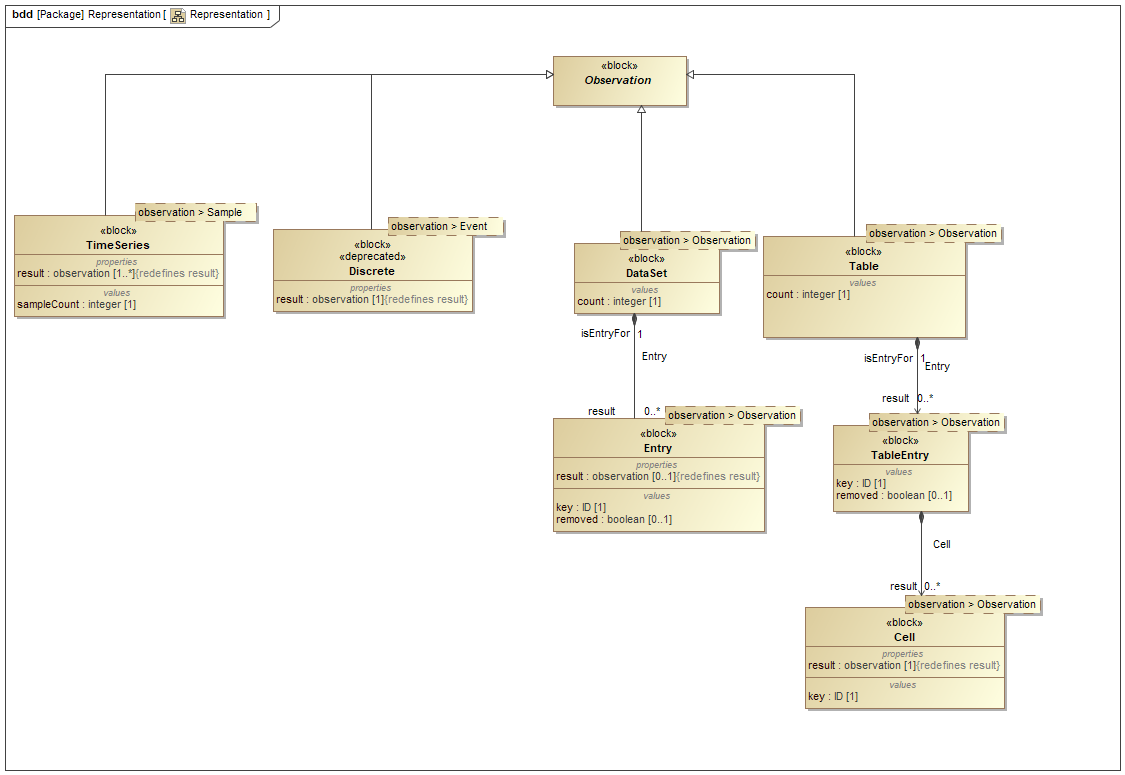
\includegraphics[width=1.0\textwidth]{figures/Representation.png}
  \caption{Representation Diagram}
  \label{fig:Representation Diagram}
\end{figure}

\FloatBarrier


Note: See \sect{Representation Schema Diagrams} for XML schema.


\subsubsection{TimeSeries}
\label{sec:TimeSeries}




A \block{DataItem} with \texttt{TIME\textunderscore SERIES} \property{representation} \textbf{MUST} have a \property{category} of \texttt{SAMPLE}.

A \textit{Time Series} \gls{observation} \textbf{MUST} have a \property{sampleCount} attribute.

\textit{Time Series} \gls{observation} \textbf{MUST} report multiple values at fixed intervals in a single \gls{observation}. At minimum, one of DataItem or \gls{observation} \textbf{MUST} specify the \property{sampleRate} in Hertz (values/second); fractional rates are permitted. When the \gls{observation} and the \block{DataItem} specify the \property{sampleRate}, the \gls{observation} \property{sampleRate} supersedes the \block{DataItem}.

The \gls{observation} \textbf{MUST} set the \property{timestamp} to the time the last value was observed. The \property{duration} \textbf{MAY} indicate the time interval from the first to the last value in the series.

\sect{Attributes of TimeSeries} defines additional attributes provided for a \block{DataItem} of \texttt{category} \texttt{SAMPLE} with a \property{representation} attribute of \texttt{TIME\textunderscore SERIES}.


\paragraph{Attributes of TimeSeries}\mbox{}
\label{sec:Attributes of TimeSeries}

\tbl{Attributes of TimeSeries} lists the attributes of \texttt{TimeSeries}.

\begin{table}[ht]
\centering 
  \caption{Attributes of TimeSeries}
  \label{table:Attributes of TimeSeries}
\tabulinesep=3pt
\begin{tabu} to 6in {|l|l|l|} \everyrow{\hline}
\hline
\rowfont\bfseries {Attribute} & {Type} & {Multiplicity} \\
\tabucline[1.5pt]{}

\property{sampleCount}[TimeSeries] & \texttt{integer} & 1 \\
\end{tabu}
\end{table}
\FloatBarrier

Descriptions for attributes of \block{TimeSeries}:

\begin{itemize}

\item \property{sampleCount}[TimeSeries] \newline The number of values given for the \block{Observation} element.
\end{itemize}



\subsubsection{Discrete}
\label{sec:Discrete}



\textit{MTConnect Version 1.5} replaced \property{representation} \texttt{DISCRETE} with a \property{discrete} attribute for \block{DataItem}.

\texttt{DISCRETE} \MUST only be used with a \block{DataItem} with a \property{category} of \texttt{EVENT}.

Each occurrence of the \gls{observation} \textbf{MAY} have the same value as the previous occurrence, and \textbf{MUST NOT} suppress duplicates.

Examples of \texttt{DISCRETE} information as follows: A \texttt{PartCount} reporting the completion of each part using a 1 to indicate completion of a single part, a \texttt{Message} that occurs each time a door opens. 




\subsubsection{DataSet}
\label{sec:DataSet}



A \block{DataItem} with \texttt{DATA\textunderscore SET} \property{representation} \textbf{MUST} have a \property{category} of \texttt{SAMPLE} or \texttt{EVENT}. 

A \gls{Data Set} \gls{observation} \textbf{MUST} have a \property{count} attribute.

\gls{Data Set} \gls{observation} reports multiple values as a set of \gls{key-value pair} where each \gls{key} \textbf{MUST} be unique. The representation of the \gls{key-value pair} is an \block{Entry}. The value of each \block{Entry} \textbf{MUST} have the same constraints and format as the \gls{observation} defined for the \texttt{VALUE} \property{representation} for the \block{DataItem} \property{type}. 

The meaning of each \block{Entry} \textbf{MAY} be provided as the \block{DataItem} \block{EntryDefinition}.


\paragraph{Attributes of DataSet}\mbox{}
\label{sec:Attributes of DataSet}

\tbl{Attributes of DataSet} lists the attributes of \texttt{DataSet}.

\begin{table}[ht]
\centering 
  \caption{Attributes of DataSet}
  \label{table:Attributes of DataSet}
\tabulinesep=3pt
\begin{tabu} to 6in {|l|l|l|} \everyrow{\hline}
\hline
\rowfont\bfseries {Attribute} & {Type} & {Multiplicity} \\
\tabucline[1.5pt]{}

\property{count}[DataSet] & \texttt{integer} & 1 \\
\end{tabu}
\end{table}
\FloatBarrier

Descriptions for attributes of \block{DataSet}:

\begin{itemize}

\item \property{count}[DataSet] \newline The number of \block{Entry} elements for the \gls{observation}.
\end{itemize}


\paragraph{Elements of DataSet}\mbox{}
\label{sec:Elements of DataSet}

\tbl{Elements of DataSet} lists the elements of \texttt{DataSet}.

\begin{table}[ht]
\centering 
  \caption{Elements of DataSet}
  \label{table:Elements of DataSet}
\tabulinesep=3pt
\begin{tabu} to 6in {|l|l|} \everyrow{\hline}
\hline
\rowfont\bfseries {Element} & {Multiplicity} \\
\tabucline[1.5pt]{}
\texttt{Entry} & 0..* \\
\end{tabu}
\end{table}
\FloatBarrier


Descriptions for elements of \block{DataSet}:

\begin{itemize}

\item \block{Entry} \newline See \sect{Entry} for details on \texttt{Entry} element for \block{DataSet}.
\end{itemize}

\paragraph{Management of Data Set Observations} \mbox{}
\label{sec:Management of Data Set Observations}

An \gls{Agent} \textbf{MUST} maintain the current state of the \gls{Data Set} as described in \citetitle{MTCPart1} \textit{Section Part 1: Management of Streaming Data Storage}.

One or more \glspl{key-value pair} \textbf{MAY} be added, removed, or changed in an \gls{observation}. An \gls{Agent} \textbf{MUST} publish the changes to one or more \glspl{key-value pair} as a single \gls{observation}. An \gls{Agent} \textbf{MUST} indicate the removal of a \gls{key-value pair} from a \gls{Data Set} using the \property{removed} attribute equal \texttt{true}.

When the \block{DataItem} \property{discrete}[DataItem] attribute is \texttt{false} or is not present, an \gls{Agent} in response to a \gls{Sample Request} \textbf{MUST} only publish the changed \gls{key-value pair} since the previous state of the \gls{Data Set}.

When the \block{DataItem} \property{discrete}[DataItem] attribute is \texttt{true}, an \gls{Agent}, in response to a \gls{Sample Request}, \textbf{MUST} report all \glspl{key-value pair} ignoring the state of the \gls{Data Set}.

When an \gls{Agent} responds to a \gls{Current Request}, the \gls{Response Document} \textbf{MUST} include the full set of \glspl{key-value pair}. If the \gls{Current Request} includes an \texttt{at} query parameter, the \gls{Agent} \textbf{MUST} provide the set of \glspl{key-value pair} at the  \gls{sequence number}.

When an \gls{observation} \gls{reset} occurs, the \gls{Data Set} \textbf{MUST} remove all \glspl{key-value pair} making the set empty. The \gls{observation} \textbf{MAY} simultaneously populate the \gls{Data Set} with new \glspl{key-value pair}. The previous entries \textbf{MUST NOT} be included and \textbf{MUST NOT} have \property{removed} attribute equal \texttt{true}.

When the \gls{observation} is \texttt{UNAVAILABLE} the \gls{Data Set} \textbf{MUST} remove all \glspl{key-value pair} making the set empty.

\subsubsection{Entry}
\label{sec:Entry}



A \gls{key-value pair} published as part of a \gls{Data Set} \gls{observation}.


\paragraph{Attributes of Entry}\mbox{}
\label{sec:Attributes of Entry}

\tbl{Attributes of Entry} lists the attributes of \texttt{Entry}.

\begin{table}[ht]
\centering 
  \caption{Attributes of Entry}
  \label{table:Attributes of Entry}
\tabulinesep=3pt
\begin{tabu} to 6in {|l|l|l|} \everyrow{\hline}
\hline
\rowfont\bfseries {Attribute} & {Type} & {Multiplicity} \\
\tabucline[1.5pt]{}

\property{key}[Entry] & \texttt{ID} & 1 \\
\property{removed}[Entry] & \texttt{boolean} & 0..1 \\
\end{tabu}
\end{table}
\FloatBarrier

Descriptions for attributes of \block{Entry}:

\begin{itemize}

\item \property{key}[Entry] \newline A unique identifier for each \gls{key-value pair}.

\item \property{removed}[Entry] \newline Boolean removal indicator of a \gls{key-value pair} that \textbf{MUST} be \texttt{true} or \texttt{false}.
\end{itemize}

\paragraph{Constraints for Entry Values}\mbox{}
\label{sec:Constraints for Entry Values}

The value of each \block{Entry} \textbf{MUST} have the same restrictions as the value of an \gls{observation} with \property{representation} of \texttt{VALUE}.

An \block{Entry} \textbf{MAY} be further constrained by the \block{DataItem} definition (see \citetitle{MTCPart2}), for example a \texttt{VariableDataSet} having a string value \textbf{MAY} have a floating-point \block{Temperature} value. A restriction \textbf{MUST NOT} be broadened or removed, for example, the value "READY" \textbf{MUST NOT} occur with a \texttt{TemperatureDataSet} constrained to floating-point numbers.

The \citetitle{MTCPart2} \block{DataItem} \block{Definition} \textbf{MAY} provide the \property{type} and \property{units} of an \block{Entry} for a \property{key}.

\subsubsection{Table}
\label{sec:Table}



A \gls{Table} represents two-dimensional sets of \glspl{key-value pair} where the \block{Entry} represents rows containing sets of \glspl{key-value pair} given by \block{Cell} elements. The \gls{Table} has the same behavior as the \gls{Data Set} for change tracking, clearing, and history. When an \block{Entry} changes. All \block{Cell} elements update at the same time; they are not tracked separately like \block{Entry}.

The meaning of each \block{Entry} and \block{Cell} \textbf{MAY} be provided as the \block{DataItem} \block{EntryDefinition} and \block{CellDefinition}.

The \block{Entry} \property{key} attribute \textbf{MUST} be the unique identity of the \block{Entry} within an \gls{observation}. The \block{Cell} \property{key} attribute \textbf{MUST} be the unique identity of the \block{Cell} within an \block{Entry}.



\paragraph{Attributes of Table}\mbox{}
\label{sec:Attributes of Table}

\tbl{Attributes of Table} lists the attributes of \texttt{Table}.

\begin{table}[ht]
\centering 
  \caption{Attributes of Table}
  \label{table:Attributes of Table}
\tabulinesep=3pt
\begin{tabu} to 6in {|l|l|l|} \everyrow{\hline}
\hline
\rowfont\bfseries {Attribute} & {Type} & {Multiplicity} \\
\tabucline[1.5pt]{}

\property{count}[Table] & \texttt{integer} & 1 \\
\end{tabu}
\end{table}
\FloatBarrier

Descriptions for attributes of \block{Table}:

\begin{itemize}

\item \property{count}[Table] \newline Represents the number of \glspl{key-value pair} represented as \block{Entry} elements.
\end{itemize}


\paragraph{Elements of Table}\mbox{}
\label{sec:Elements of Table}

\tbl{Elements of Table} lists the elements of \texttt{Table}.

\begin{table}[ht]
\centering 
  \caption{Elements of Table}
  \label{table:Elements of Table}
\tabulinesep=3pt
\begin{tabu} to 6in {|l|l|} \everyrow{\hline}
\hline
\rowfont\bfseries {Element} & {Multiplicity} \\
\tabucline[1.5pt]{}
\texttt{TableEntry} (organized by \block{Entry}) & 0..* \\
\end{tabu}
\end{table}
\FloatBarrier


Descriptions for elements of \block{Table}:

\begin{itemize}

\item \block{Entry} \newline See \sect{TableEntry} for details on \texttt{Entry} element for \block{Table}.
\end{itemize}



\subsubsection{TableEntry}
\label{sec:TableEntry}



A \gls{key-value pair} published as part of a \gls{Table} \gls{observation}.

Note: Represented as \block{Entry} in XML.


\paragraph{Attributes of TableEntry}\mbox{}
\label{sec:Attributes of TableEntry}

\tbl{Attributes of TableEntry} lists the attributes of \texttt{TableEntry}.

\begin{table}[ht]
\centering 
  \caption{Attributes of TableEntry}
  \label{table:Attributes of TableEntry}
\tabulinesep=3pt
\begin{tabu} to 6in {|l|l|l|} \everyrow{\hline}
\hline
\rowfont\bfseries {Attribute} & {Type} & {Multiplicity} \\
\tabucline[1.5pt]{}

\property{key}[TableEntry] & \texttt{ID} & 1 \\
\property{removed}[TableEntry] & \texttt{boolean} & 0..1 \\
\end{tabu}
\end{table}
\FloatBarrier

Descriptions for attributes of \block{TableEntry}:

\begin{itemize}

\item \property{key}[TableEntry] \newline A unique identifier for each \gls{key-value pair}.

\item \property{removed}[TableEntry] \newline Boolean removal indicator of a \gls{key-value pair} that \textbf{MUST} be \texttt{true} or \texttt{false}.
\end{itemize}


\paragraph{Elements of TableEntry}\mbox{}
\label{sec:Elements of TableEntry}

\tbl{Elements of TableEntry} lists the elements of \texttt{TableEntry}.

\begin{table}[ht]
\centering 
  \caption{Elements of TableEntry}
  \label{table:Elements of TableEntry}
\tabulinesep=3pt
\begin{tabu} to 6in {|l|l|} \everyrow{\hline}
\hline
\rowfont\bfseries {Element} & {Multiplicity} \\
\tabucline[1.5pt]{}
\texttt{Cell} & 0..* \\
\end{tabu}
\end{table}
\FloatBarrier


Descriptions for elements of \block{TableEntry}:

\begin{itemize}

\item \block{Cell} \newline See \sect{Cell} for details on \block{Cell} element for \block{TableEntry}.
\end{itemize}



\subsubsection{Cell}
\label{sec:Cell}



An element representing a \gls{key-value pair} published as part of an \block{Entry}.


\paragraph{Attributes of Cell}\mbox{}
\label{sec:Attributes of Cell}

\tbl{Attributes of Cell} lists the attributes of \texttt{Cell}.

\begin{table}[ht]
\centering 
  \caption{Attributes of Cell}
  \label{table:Attributes of Cell}
\tabulinesep=3pt
\begin{tabu} to 6in {|l|l|l|} \everyrow{\hline}
\hline
\rowfont\bfseries {Attribute} & {Type} & {Multiplicity} \\
\tabucline[1.5pt]{}

\property{key}[Cell] & \texttt{ID} & 1 \\
\end{tabu}
\end{table}
\FloatBarrier

Descriptions for attributes of \block{Cell}:

\begin{itemize}

\item \property{key}[Cell] \newline A unique identifier for each \gls{key-value pair}.
\end{itemize}

\paragraph{Constraints for Cell Values}\mbox{}
\label{sec:Constraints for Cell Values}

The value of each \block{Cell} \textbf{MUST} have the same restrictions as the value of an \gls{observation} with \property{representation} of \texttt{VALUE}.

An \block{Cell} \textbf{MAY} be further constrained by the \block{DataItem} definition (see \citetitle{MTCPart2}), for example a \texttt{VariableDataSet} having a string value \textbf{MAY} have a floating-point \block{Temperature} value. A restriction \textbf{MUST NOT} be broadened or removed, for example, the value \texttt{READY} \textbf{MUST NOT} occur with a \texttt{TemperatureDataSet} constrained limited to floating-point numbers.

The \citetitle{MTCPart2} \block{DataItem} \block{Definition} \textbf{MAY} provide the \property{type} and \property{units} of a \block{Cell} for a \property{key}.
